% ============================================================
%  UROLOGÍA INTRAOPERATORIA
%  Licenciatura en Imagenología --- UdelaR
%  Fuente: clase Lic. Matías Prado, Imagenología Especializada I
% ============================================================

\chapter{Urologia Intraoperatoria}


% ============================================================
%  PUNTOS CLAVE PARA EL EXAMEN ORAL
% ============================================================
\begin{cajakeypoints}
\textbf{\color{azulprincipal} Puntos clave para el examen oral}
\begin{itemize}[noitemsep, topsep=2pt]
  \item El licenciado en imagenología es \textbf{personal no estéril}: no puede tocar al cirujano, instrumentista ni la mesa estéril.
  \item \textbf{Catéter Doble J}: acceso retrógrado vía uretra; paciente en decúbito supino con piernas en posición ginecológica (independiente del género).
  \item \textbf{Nefrostomía percutánea}: acceso anterógrado a través de la piel; paciente en decúbito prono; arco en C contralateral al riñón a puncionar.
  \item \textbf{Litotricia endoscópica}: misma posición que Doble J; para cálculos ureterales; sin rayos durante la fragmentación.
  \item \textbf{Litotricia percutánea (nefrolitotomía)}: paciente supino lateralizado con el riñón a trabajar hacia arriba; arco contralateral al riñón afectado.
  \item Los cálculos menores a \textbf{5 mm} se expulsan solos; los mayores a \textbf{8 mm} requieren litotricia percutánea. Entre 5--8 mm: litotricia endoscópica.
  \item Las tres \textbf{estrecheces ureterales} (sitios más frecuentes de cálculos): unión pieloureteral, cruce con vasos ilíacos, y unión ureterovesical.
  \item El contraste utilizado en todos los procedimientos es \textbf{yodado}.
  \item El \textbf{uréter totalmente dilatado} es signo de patología (obstrucción); la ausencia intermitente del uréter en imágenes es normal (peristaltismo).
\end{itemize}
\end{cajakeypoints}

\vspace{1em}

% ============================================================
%  ANATOMÍA DE REFERENCIA	
% ============================================================
\section*{Anatomía de referencia}

\begin{cajadefinicion}
El \textbf{aparato urinario} está constituido por dos riñones, los uréteres, la vejiga y la uretra. Mantiene el equilibrio ácido-base y el balance hidrosalino eliminando desechos metabólicos.
\end{cajadefinicion}

Los riñones son órganos \textbf{retroperitoneales} ubicados entre D12 y L3. El riñón derecho se encuentra más descendido que el izquierdo por la impresión hepática. Anatómicamente no están en el plano sagital: presentan una inclinación de aproximadamente \textbf{20 grados}, lo que tiene implicancia directa en las proyecciones oblicuas durante los procedimientos.
\clearpage

Los uréteres transportan la orina mediante \textbf{ondas peristálticas}. Presentan tres puntos anatómicos de estrechez donde los cálculos se atascan con mayor frecuencia:

\begin{itemize}[noitemsep]
  \item Unión pieloureteral.
  \item Sitio de entrecruzamiento con los vasos ilíacos.
  \item Unión ureterovesical (porción intramural en la cara posterolateral de la vejiga).
\end{itemize}

\subsection*{Personal en block quirúrgico}

El equipo quirúrgico se divide en personal \textbf{estéril} (cirujano, ayudantes, instrumentista: túnica estéril + lavado quirúrgico + guantes) y personal \textbf{no estéril} (licenciado en imagenología, anestesista, auxiliar de enfermería: casaca, pantalón, gorro, tapaboca). El licenciado \textbf{nunca debe tocar} al personal estéril ni la mesa del instrumentista para no contaminar el campo.

% ============================================================
%  CLASIFICACIÓN DE LOS PROCEDIMIENTOS
% ============================================================
\section*{Clasificación de los procedimientos}

\subsection*{Por tipo de acceso y objetivo}

{\renewcommand{\arraystretch}{1.35}
\begin{center}
\begin{tabular}{>{\bfseries}p{3.5cm} p{4.5cm} p{6cm}}
\hline
Procedimiento & Acceso & Objetivo principal \\
\hline
Catéter Doble J & Retrógrado (vía uretra) & Bypass ureteral ante obstrucción o injuria temporal. \\[0.5em]
\hline
Nefrostomía percutánea & Anterógrado (vía piel) & Drenaje externo del riñón obstruido mediante bolsa colectora. \\[0.5em]
\hline
Litotricia endoscópica & Retrógrado (vía uretra) & Fragmentación y extracción de cálculos ureterales ($<$8 mm). \\[0.5em]
\hline
Litotricia percutánea & Anterógrado (vía piel) & Extracción de cálculos renales grandes ($>$8 mm) en pelvis renal. \\
\hline
\end{tabular}
\end{center}

\clearpage

% ============================================================
%  PROCEDIMIENTO 1: CATÉTER DOBLE J
% ============================================================
\section*{Catéter Doble J}

\begin{cajadefinicion}
El \textbf{catéter Doble J} es un tubo fino, flexible y fenestrado que se coloca internamente entre la pelvis renal y la vejiga para asegurar el drenaje de orina ante obstrucciones, lesiones ureterales o como protección posquirúrgica. Sus dos extremos curvados en ``J'' lo fijan en posición. Es un dispositivo \textbf{temporal}.
\end{cajadefinicion}


\subsection*{Indicaciones}
Obstrucción ureteral por cálculo, tumor o estenosis; protección del uréter tras cirugía; tratamiento coadyuvante de litiasis (se deja tras litotricia para favorecer cicatrización de la pared ureteral).

\subsection*{Posición del paciente y distribución de sala}

\begin{itemize}[noitemsep]
  \item Paciente: \textbf{decúbito supino}, piernas en \textbf{posición ginecológica} (independiente del género; el ureteroscopio accede igualmente en ambos sexos).
  \item Cola del paciente pegada al \textbf{borde inferior de la mesa} para permitir que el arco en C llegue hasta el abdomen superior.
  \item Cirujano y ayudante: entre las piernas del paciente.
  \item Instrumentista: a los pies del paciente.
  \item Rack de ureteroscopio: lateral al cirujano.
  \item \textbf{Licenciado en imagenología}: ingresa \textbf{perpendicular}, por el costado que queda libre (opuesto al rack). El monitor de RX se coloca del lado del licenciado.
  \item La entrada del arco en C es \textbf{independiente del riñón} en estudio.\\
\end{itemize}

\begin{cajariesgo}
\textbf{Obstáculos a anticipar:} piernas del paciente, balde debajo de la mesa (el ureteroscopio irriga suero continuamente), base y escalón de la mesa, brazos del paciente, portasueros. Verificar la sala \textbf{antes} de que el paciente esté dormido.
\end{cajariesgo}

\subsection*{Secuencia del procedimiento}

\begin{enumerate}[noitemsep]
  \item El cirujano introduce el \textbf{ureteroscopio} por la uretra hasta la vejiga.
  \item \textbf{Enfoque inicial} del licenciado: frente centrado en vejiga, siguiendo la punta del catéter hasta el meato ureteral.
  \item \textbf{Pielografía retrógrada}: se inyecta contraste yodado a través del catéter recto desde vejiga hacia pelvis renal (sentido contrario a la orina; de ahí el término \textit{retrógrada}). Permite visualizar anatomía, cálculos y estado del uréter.
  \item Se asciende siguiendo la subida del cirujano: el licenciado \textbf{acompaña} el catéter desde vejiga hasta pelvis renal.
  \item Control en pelvis renal: se verifica que la \textbf{guía metálica} esté correctamente posicionada.
  \item Se asciende el \textbf{Doble J} a través de la guía. Se retira la guía; queda solo el catéter.
  \item \textbf{Control final de ambos rulos}: un disparo en pelvis renal (extremo proximal) y un disparo en vejiga (extremo distal). Fin del procedimiento.\\
\end{enumerate}

\begin{cajakeypoints}
\textbf{Concepto clave:} Es el procedimiento urológico más simple y breve ($\sim$10 minutos). No requiere angulaciones especiales ni sustracción digital. Ideal para iniciarse en block quirúrgico.
\end{cajakeypoints}

\begin{figure}[h]
    \centering
    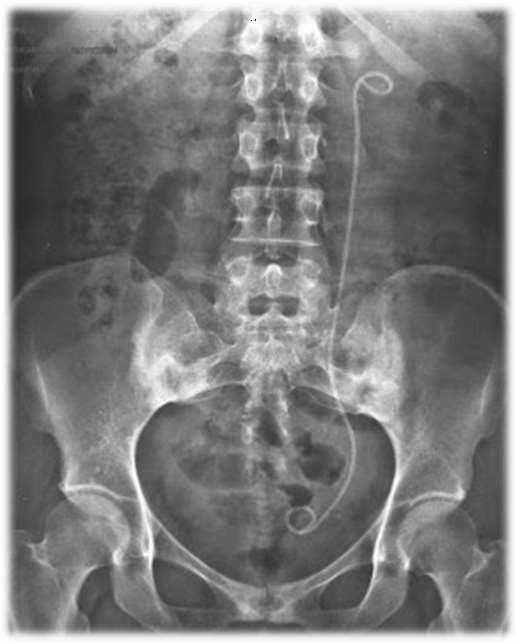
\includegraphics[width=0.5\linewidth]{imagenes/dobleJ.png}
    \caption{Doble J}
    \label{fig:Doble J}
\end{figure}

\clearpage
% ============================================================
%  PROCEDIMIENTO 2: NEFROSTOMÍA PERCUTÁNEA
% ============================================================
\section*{Nefrostomía Percutánea}

\begin{cajadefinicion}
La \textbf{nefrostomía percutánea} consiste en la colocación de un catéter flexible a través de la piel hasta la pelvis renal para drenar orina hacia una bolsa colectora externa. Se indica cuando la obstrucción ureteral no puede resolverse por vía retrógrada o requiere descompresión urgente.
\end{cajadefinicion}

\subsection*{Indicaciones}
Obstrucción ureteral que compromete la función renal, genera dolor o fiebre; preparación previa a litotricia percutánea; obstrucciones no resolubles por vía endoscópica.

\subsection*{Posición del paciente y distribución de sala}

\begin{itemize}[noitemsep]
  \item Paciente: \textbf{decúbito prono} (boca abajo).
  \item Cirujano y ayudantes: del lado del \textbf{riñón a puncionar}.
  \item \textbf{Licenciado en imagenología}: ingresa perpendicular, por el \textbf{lado contralateral} al riñón afectado (lado libre). Si se trabaja el riñón izquierdo, el arco entra por la derecha.
\end{itemize}

\subsection*{Enfoques complementarios}

Los riñones tienen una inclinación de $\sim$20° respecto al plano sagital. Un frente estricto los muestra en oblicua. Para verlos \textbf{de frente} se requiere una oblicua:

{\renewcommand{\arraystretch}{1.35}
\begin{center}
\begin{tabular}{>{\bfseries}p{3cm} p{5.5cm} p{5.5cm}}
\hline
Posición del arco & Técnica & Indicación \\
\hline
PA (boca abajo) & Oblicua \textbf{contralateral}: intensificador se aleja del licenciado, hacia el lado de los médicos. & Visualizar el riñón de frente durante la punción. \\[0.5em]
\hline
AP (hipotético) & Oblicua \textbf{homolateral}: intensificador hacia el licenciado. & Solo orientativo; el procedimiento es siempre en prono. \\
\hline
\end{tabular}
\end{center}
}

\clearpage

\subsection*{Secuencia del procedimiento}

\begin{enumerate}[noitemsep]
  \item \textbf{Enfoque inicial}: frente centrado en el riñón de interés. Referencias anatómicas: columna vertebral (límite medial) y última costilla (límite superior). Riñones entre D12 y L3.
  \item El cirujano realiza la \textbf{punción renal} con aguja de punta abierta. La salida de orina por la punta confirma que está en pelvis renal.

\begin{figure}[h]
    \centering
    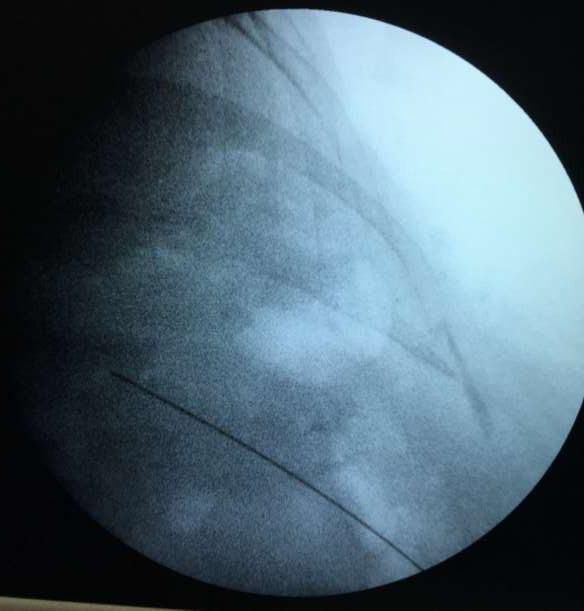
\includegraphics[width=0.5\linewidth]{imagenes/puncionRenal.png}
    \caption{Punción renal}
    \label{fig:puncion}
\end{figure}

  \item \textbf{Pielografía anterógrada}: se inyecta contraste yodado a través de la aguja. Se opacifican cálices, pelvis renal y uréter (sentido de la orina; de ahí \textit{anterógrada}).

\begin{figure}[h]
    \centering
    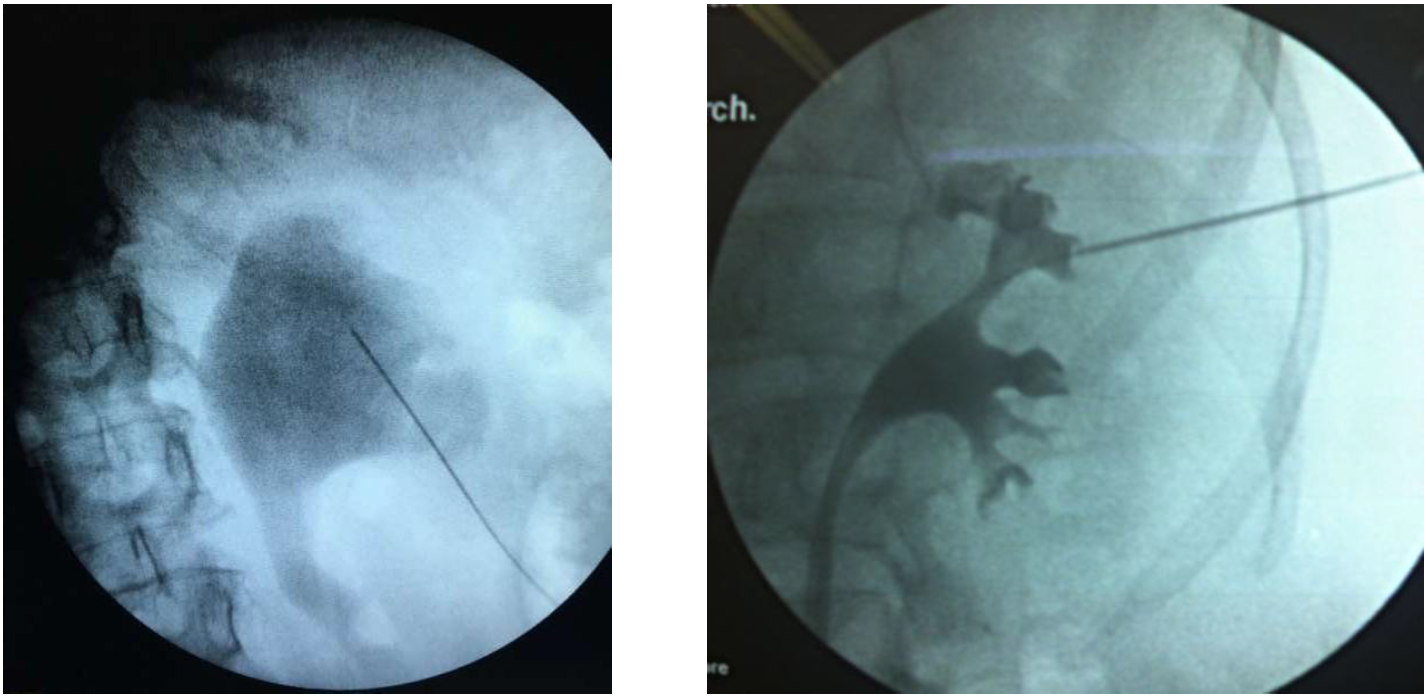
\includegraphics[width=1\linewidth]{imagenes/anterograda.png}
    \caption{Pielografia anterograda}
    \label{fig:pielografia}
\end{figure}

\clearpage


  \item Se pasa la \textbf{guía metálica} a través del catéter de punción.

  \begin{figure}[h]
      \centering
      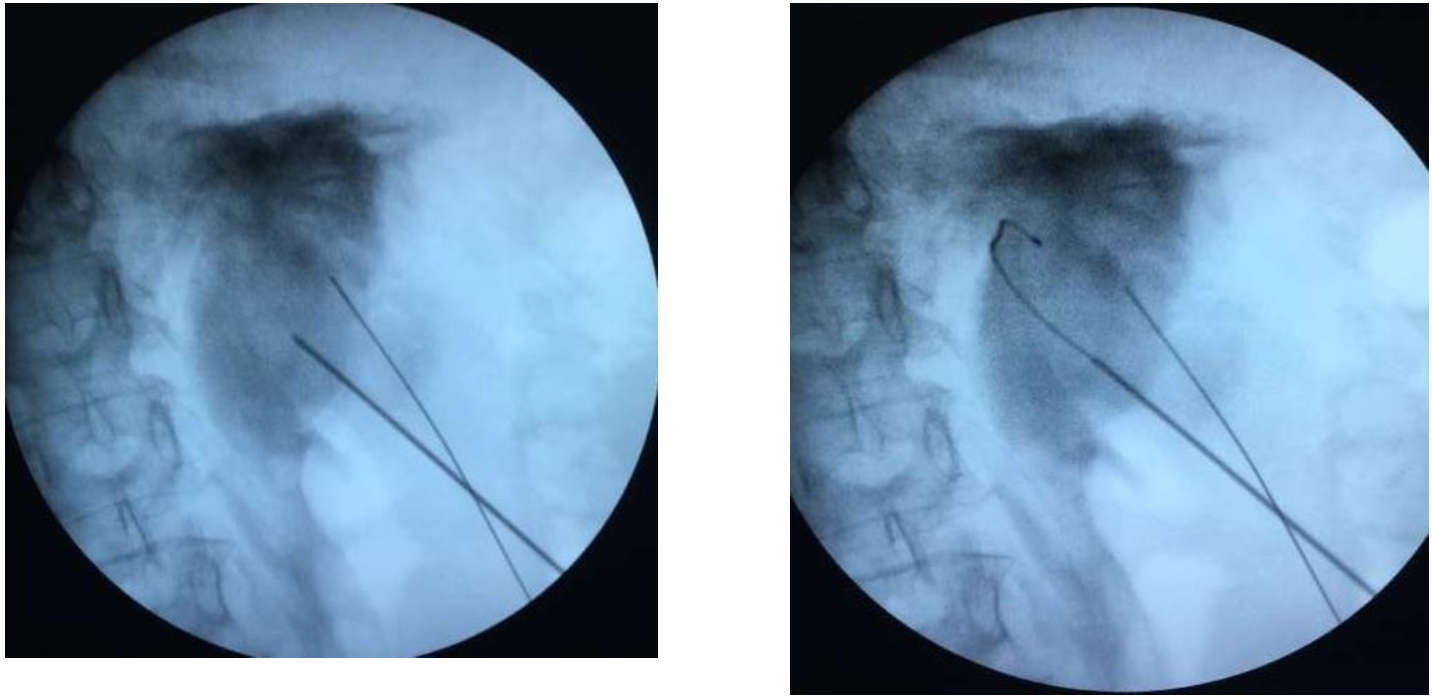
\includegraphics[width=1\linewidth]{imagenes/guia.png}
      \caption{Guía metalica}
      \label{fig:guia}
  \end{figure}

  
  \item Se colocan \textbf{dilatadores} sucesivos sobre la guía para ampliar el trayecto percutáneo.

\begin{figure}[htbp]
    \centering
    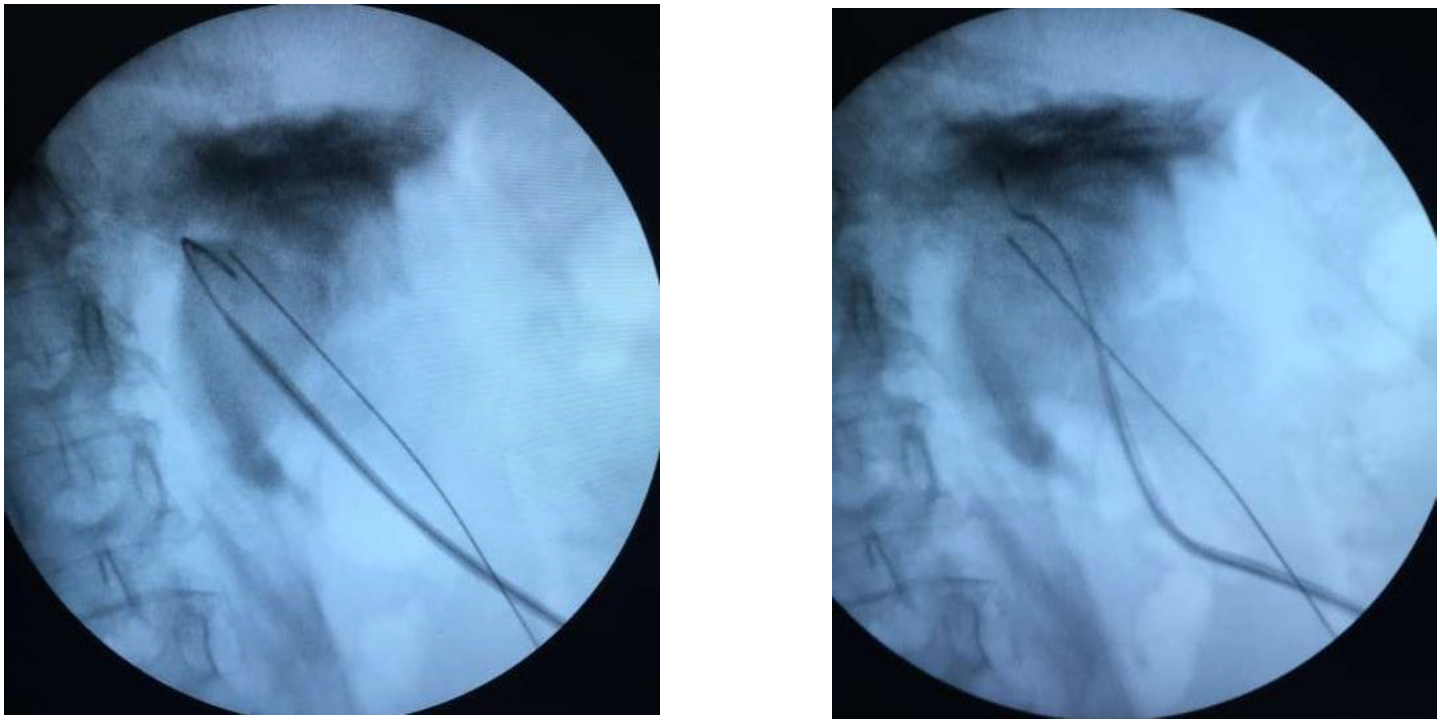
\includegraphics[width=1\linewidth]{imagenes/dilatadores.png}
    \caption{Dilatadores}
    \label{fig:Dilatadores}
\end{figure}
  
  \clearpage
  
  \item Se coloca la \textbf{sonda de nefrostomía} a través de la guía. Se retiran guía y dilatador.
  
  \begin{figure}[htbp]
  	\centering
  	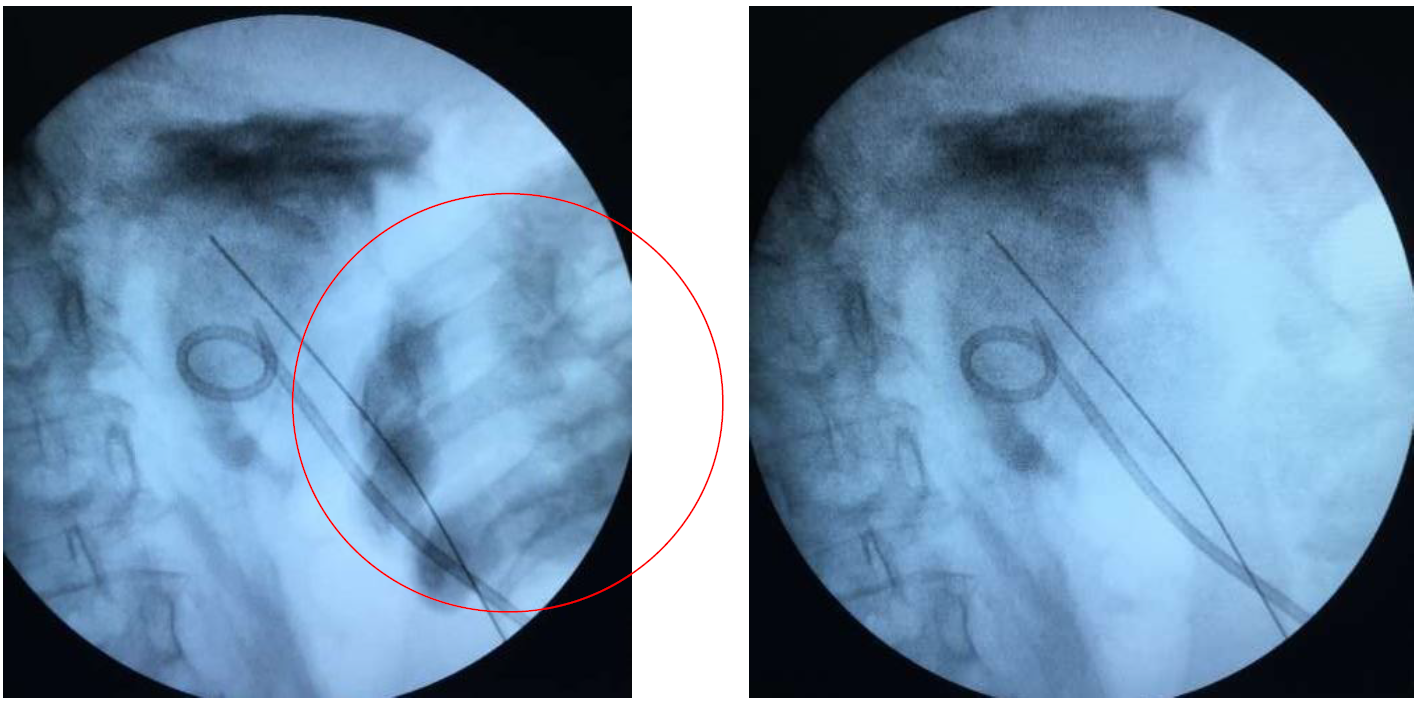
\includegraphics[width=1\linewidth]{screenshot001}
  	\caption{Sonda de nefrostomia}
  	\label{fig:sondanefrostomia}
  \end{figure}
  
  \item \textbf{Pielografía de control final}: se verifica la correcta posición del catéter y la permeabilidad del sistema.
  
\end{enumerate}

  \begin{figure}[h]
	\centering
	\includegraphics[width=0.5\linewidth]{"pielografia final"}
	\caption{Pielografia final}
	\label{fig:pielografia-final}
\end{figure}



\clearpage

\begin{cajariesgo}
\textbf{Importante:} No disparar rayos cuando el cirujano tenga las manos dentro del campo renal. Coordinarse verbalmente antes de cada disparo. El licenciado no se mueve una vez centrado en el riñón; el procedimiento completo se realiza en la misma posición.
\end{cajariesgo}

.\\

\begin{cajakeypoints}
\textbf{Concepto clave:} Radiológicamente es más simple que el Doble J (posición fija durante todo el procedimiento), pero el tiempo total es mayor por la dificultad de la punción percutánea, que puede demandar múltiples intentos del cirujano.
\end{cajakeypoints}

\clearpage
% ============================================================
%  PROCEDIMIENTO 3: LITOTRICIA
% ============================================================
\section*{Litotricia}

\begin{cajadefinicion}
La \textbf{litotricia} es un procedimiento que utiliza ondas de choque para fragmentar cálculos del aparato urinario (riñón, uréter o vejiga) y permitir su eliminación. Solo requieren apoyo radiológico las modalidades \textbf{ureteral} y \textbf{renal}; la vesical se guía exclusivamente por endoscopía.
\end{cajadefinicion}

Estudios previos: ecografía; si no es concluyente, \textbf{Urotac} (TC sin contraste). El 90\% de los cálculos son radiopacos y se visualizan sin contraste. El contraste taparía el cálculo, por lo que se evita en la mayoría de los casos.

\subsection*{Litotricia endoscópica (ureteral)}

\textbf{Indicación:} cálculos ureterales. Posición del paciente y del arco en C: \textbf{idéntica al Doble J} (decúbito supino, piernas en posición ginecológica; licenciado perpendicular por el costado libre).

\begin{enumerate}[noitemsep]
  \item \textbf{Pielografía retrógrada}: igual que en el Doble J. Se localiza el cálculo.
  \item El licenciado acompaña la subida del ureteroscopio \textbf{hasta el cálculo}.
  \item Fragmentación con ondas de choque o láser: \textbf{sin rayos} (el cirujano trabaja por visión endoscópica directa).
  \item Extracción de fragmentos con \textbf{canastilla Dormia} o aspiración.
  \item \textbf{Pielografía de control}: verifica ausencia de cálculos residuales y permeabilidad ureteral.
  \item En la mayoría de los casos se deja un \textbf{Doble J} temporal para proteger el uréter durante la cicatrización (se retira ambulatoriamente en policlínica, sin rayos).
\end{enumerate}

\subsection*{Litotricia percutánea (nefrolitotomía percutánea)}

\textbf{Indicación:} cálculos renales grandes ($>$8 mm) o cuando la vía endoscópica no es viable.

\textbf{Posición del paciente:} \textbf{decúbito supino lateralizado}, con el riñón a trabajar hacia arriba. El licenciado ingresa perpendicular, por el \textbf{lado contralateral} (el que queda abajo). Mismo principio que en nefrostomía percutánea.

\begin{enumerate}[noitemsep]
  \item El cirujano coloca una \textbf{sonda en vejiga} para ocluir el flujo y facilitar el trabajo (no requiere acción del licenciado).
  \item \textbf{Punción renal}: igual que en nefrostomía. El licenciado centra el campo en el riñón y permanece ahí durante todo el procedimiento.
  \item \textbf{Dilatación} del trayecto percutáneo.
  \item Introducción del \textbf{nefroscopio} a través del trayecto dilatado.
  \item Fragmentación de cálculos con ondas de choque.
  \item Extracción de fragmentos.
  \item \textbf{Pielografía anterógrada final}: verifica limpieza de la pelvis renal.
  \item Se deja un \textbf{set de nefrostomía} temporal para el período de recuperación.
\end{enumerate}

\clearpage

\begin{cajakeypoints}
\textbf{Proyección de perfil (complementaria):} Girar el arco en C a 90° a pedido del cirujano. El perfil informa la \textbf{altura de trabajo} del arco; establecida esa altura, mantenerla fija para todo el procedimiento (tanto en frente como en perfil). Avisar al cirujano antes de girar el arco para que se retire del campo.
\end{cajakeypoints}

.\\


\begin{cajariesgo}
\textbf{Posición correcta del paciente:} La zona de trabajo (pelvis renal) debe quedar libre hacia arriba y hacia abajo para poder realizar tanto el frente como el perfil. Si el paciente no está bien posicionado, corregirlo \textbf{antes} de iniciar el procedimiento. No tener vergüenza en solicitarlo: el resto del equipo no sabe lo que el licenciado necesita mostrar.
\end{cajariesgo}

% ============================================================
%  TABLA COMPARATIVA DE LOS CUATRO PROCEDIMIENTOS
% ============================================================
\section*{Tabla comparativa de los procedimientos}

{\renewcommand{\arraystretch}{1.35}
	\begin{center}
		\begin{tabular}{>{\bfseries}p{3cm} >{\centering}p{2.8cm} >{\centering}p{2.8cm} >{\centering}p{2.8cm} >{\centering\arraybackslash}p{2.8cm}}
			\hline
			\textbf{Criterio} & \textbf{Doble J} & \textbf{Nefrostomía} & \textbf{Litotricia endosc.} & \textbf{Litotricia percutánea} \\
			\hline
			Posición paciente & Supino + ginecológica & Decúbito prono & Supino + ginecológica & Supino lateralizado \\[0.5em]
			\hline
			Acceso & Retrógrado (uretra) & Anterógrado (piel) & Retrógrado (uretra) & Anterógrado (piel) \\[0.5em]
			\hline
			Lado del licenciado & Costado libre (cualquiera) & Contralateral al riñón & Costado libre (cualquiera) & Contralateral al riñón \\[0.5em]
			\hline
			Pielografía & Retrógrada & Anterógrada & Retrógrada + control final & Anterógrada final \\[0.5em]
			\hline
			Duración aprox. & $\sim$10 min & 30--60 min & 20--40 min & 60--90 min \\[0.5em]
			\hline
			Complejidad Lic. & Baja & Muy baja (posición fija) & Baja & Baja (posición fija) \\
			\hline
		\end{tabular}
	\end{center}
}

\clearpage
% ============================================================
%  ESQUEMA MENTAL --- REPASO FINAL
% ============================================================
\section*{Esquema Mental --- Repaso Final}

\begin{cajakeypoints}
\begin{center}
\textbf{\color{azulprincipal}
  Obstrucción ureteral $\rightarrow$ elegir vía $\rightarrow$ retrógrada (endoscópica) o anterógrada (percutánea)}\\[0.4em]
\textbf{\color{naranjadestacado}
  Si el paciente está boca arriba con piernas en posición ginecológica: entro por el costado libre. Si está boca abajo o lateralizado: entro por el lado contralateral al riñón afectado.}\\[0.3em]
Cálculo $<5$ mm: expulsión espontánea \quad $5$--$8$ mm: litotricia endoscópica \quad $>8$ mm: litotricia percutánea\\[0.3em]
90\% de cálculos son radiopacos $\to$ Urotac sin contraste \quad Contraste utilizado: yodado\\[0.3em]
\textbf{Doble J:} cateterismo $\to$ pielografía retrógrada $\to$ guía metálica $\to$ ascenso DJ $\to$ control ambos rulos\\[0.2em]
\textbf{Nefrostomía:} punción renal $\to$ pielografía anterógrada $\to$ guía $\to$ dilatadores $\to$ catéter $\to$ pielografía final\\[0.2em]
\textbf{Litotricia endosc.:} igual que DJ hasta cálculo $\to$ ondas (sin rayos) $\to$ extracción $\to$ pielografía control $\to$ DJ\\[0.2em]
\textbf{Litotricia percutánea:} sonda vejiga $\to$ punción $\to$ dilatación $\to$ nefroscopio $\to$ fragmentación $\to$ extracción $\to$ pielografía anterógrada $\to$ nefrostomía\\
\end{center}
\end{cajakeypoints}

\vspace{1em}
\hrule
\vspace{0.5em}
{\footnotesize \textit{Fuente: material de clase --- Doc. Asis. Lic. Matías Prado,
  Imagenología Especializada I, UdelaR 2026.}}